\chapter{A Programação Linear e as suas Aplicações}

\section{Introdução}
Na pesquisa operacional, a programação linear é uma das técnicas mais utilizadas em problemas de otimização. Os problemas de programação linear geralmente buscam a distribuição eficiente de recursos limitados para atender um determinado objetivo, por isso suas aplicações estão presentes em diversas áreas como computação, administração, indústria e transporte \cite{Engecom}.

Um problema de programação linear é expresso através de um modelo que é composto por equações e inequações lineares. Esse tipo de problema busca a distribuição eficiente de recursos com restrições para alcançar um objetivo, em geral, maximizar lucros ou minimizar custos. Em um problema de programação linear esse objetivo é expresso através de uma equação linear denominada função objetivo. Para a formulação do problema, é necessário também definir os recursos necessários e em que proporção são requeridos. Essas informações são expressas em equações ou inequações lineares, uma para cada recurso. Esse conjunto de equações ou inequações é denominado restrições do modelo \cite{Engecom}.

\section{Descrição do Problema de Programação Linear}
O modelo de um problema de programação linear normalmente é apresentado em uma das formas a seguir \cite{Passos}:

$\\Max\ z = c^{T}x \\\\s.a.\left\{\begin{matrix}
Ax\leq b\\x\geq 0 
\end{matrix}\right.$  

ou  

$\\Min\ z = c^{T}x \\\\s.a.\left\{\begin{matrix}
Ax\geq  b\\x\geq 0 
\end{matrix}\right.$

Um problema de programação linear com até três variáveis pode ser representado graficamente utilizando três eixos cartesianos. Os problemas com duas variáveis podem ainda ser facilmente resolvidos por meio da representação gráfica \cite{Passos}. 

A seguir é apresentado um problema com duas variáveis e sua representação. Apesar de, na prática os problemas de programação linear possuir um número de variáveis muito maior que dois ou três, a visualização gráfica de modelo, mesmo que simples, contribui para o entendimento dos métodos de resolução apresentados nas seções a seguir.
No problema exemplo, uma empresa, que fabrica vários produtos, deseja maximizar o lucro na vendo de 2 desses produtos \cite{Hillier}.

$\\Maximize\ z=3x_{1}+5x_{2}\\
Sujeito\ a\\$
\begin{eqnarray*}
        1x_{1}\leq 4 (a)\\
              2x_{2}\leq (b)\\
        3x_{1}+2x_{2}\leq 8 (c)\\
         x_{1}\geq 0, x_{2}\geq 0
\end{eqnarray*}

Onde, 
\begin{itemize}
\item \textbf {$x_{1}$} representa a quantidade do produto 1 produzido em uma semana
\item \textbf {$x_{2}$} representa a quantidade do produto 2 produzido em uma semana
\item \textbf {$z$} representa o lucro total por semana de produção desses dois produtos (em milhões de dólares), sendo o lucro do produto 1 de 3 milhões e o do produto 2 de 5 milhões.
\end{itemize}

E as restrições representam as restrições de tempo de cada máquina utilizada no processo de produção,
\begin{itemize}
\item A equação \textbf {(a)} garante que, durante o processo de produção, cada produto 1 necessita de 1 hora na máquina 1, e a máquina só tem disponível 4 horas por semana
\item A equação \textbf {(b)} garante que, durante o processo de produção, cada produto 2 necessita de 2 horas na máquina 2, e a máquina só tem disponível 12 horas por semana
\item A equação \textbf {(c)} garante que, durante o processo de produção, cada produto 1 necessita de 3 horas na máquina 3, e cada produto 2 necessita de 2 horas na máquina 3, e a máquina só tem disponível 8 horas por semana
\end{itemize}

Graficamente representado o problema ficaria da seguinte forma:
\begin{center}
	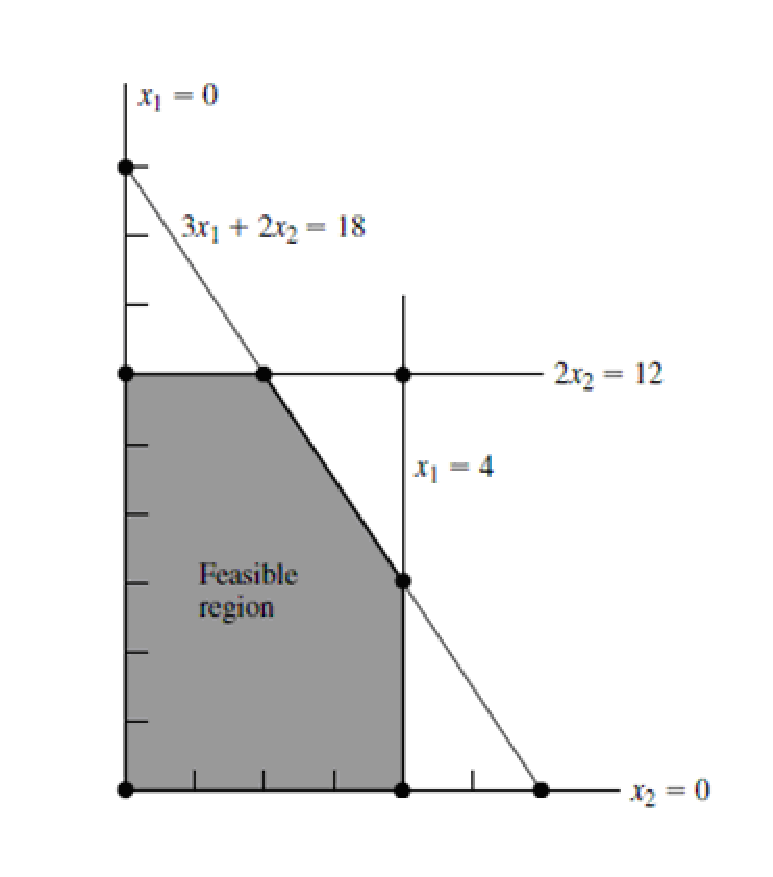
\includegraphics[scale=1.00]{graficos/simplex_grafico}
	\captionof{figure}{Representação gráfica de um Problema de Programação Linear de duas variáveis}
\end{center}

Onde cada reta representa uma restrição do modelo, e a área cinza representa a região viável, ou seja nessa área estão contidas os valores viáveis de $x_{1}$ e $x_{2}$ para a maximização do lucro.

Os métodos para resolução problemas de programação linear buscam esses valores de $x_{1}$ e $x_{2}$  para determinação da solução ótima.

\section{Métodos de Solução}
Entre os métodos mais famosos para a resolução de problemas de programação linear estão o método simplex  e o método de pontos interiores. 
Depois da apresentação do método simplex,outros métodos com diferentes abordagens foram propostos \cite{Todd}. Porém, dentre os métodos existentes apenas o método de pontos interiores é atualmente competitivo em relação ao método simplex \apud{Bixby}{Munari}. 
A principal diferença entre esse dois métodos é o que o método simplex caminha pelos vértices da região viável, enquanto o método de pontos interiores caminha pelo interior da região viável \cite{MaculanPI}. Além disso, uma outra diferença é que o simplex exige muitas iterações com cálculos simples, enquanto o método de pontos interiores poucas iterações são exigidas, porém com cálculos mais elaborados.
Apesar das vantagens do método de pontos interiores em relação ao método estudado neste trabalho, o método simplex possui melhor desempenho na resolução de problemas de pequeno porte em relação ao método de pontos interiores, tornando-se um método indispensável em ferramentas de programação linear.

\subsection{Método Simplex}
O método simplex é um dos algoritmos mais populares para a resolução de problemas de programação linear. Surgiu a mais de 60 anos atrás e foi proposto por George Dantzig.  

É um método iterativo, e sua ideia principal consiste no fato de que a cada iteração uma nova solução é encontrada, sempre melhor que a anterior até o ponto em que a solução ótima é obtida. Outra característica do método é o fato de ser matricial, ou seja, os dados a serem calculados são armazenados em matrizes.  

Com a utilização do método foi percebido que a cada iteração do método simplex eram requeridos muitos cálculos sobre valores que nem sempre importavam para a iteração seguinte, fato que do ponto de vista computacional tornaria o método ineficiente. Esse método é chamado de método simplex padrão ou tabular. A partir desse fato foi desenvolvido o método simplex revisado visando a resolução de problemas de programação linear computacionalmente.

O presente trabalho tem foco no método simplex revisado e suas variantes.

\subsection{Método de Pontos Interiores}
Em 1984, Karmarkar revolucionou a área de programação linear com a publicação de um algoritmo de complexidade polinomial que apresentou bom desempenho quando aplicado a problemas práticos \cite{MaculanPI}. Essa publicação deu origem a um novo campo de pesquisa, chamado de método dos pontos interiores. 

O método de pontos interiores tem como principal característica a de realizar a busca por soluções no interior da região viável do problema, até encontrar a solução ótima \cite{Pinto}.
Em teoria, o método de pontos interiores é melhor que o método simplex, principalmente quando se leva em conta o critério de complexidade de pior caso. O método de pontos interiores possui complexidade epolinomial, enquanto o método simplex possui complexidade exponencial No entanto, na prática ambos os métodos concorrem até hoje. Já que o sucesso do método depende da estrutura dos problemas, da esparsidade \footnote{Quando uma matriz possui uma grande proporção de elementos nulos diz-se que é uma matriz esparsa \cite{Munari}.} e da arquitetura dos computadores \cite{MaculanPI}.

\section{Aplicações Práticas}
Um problema de programação linear, como já dito anteriormente, busca a otimização na distribuição de recursos sujeitos a restrições. Por isso é considerada uma poderosa ferramenta de apoio a decisão \cite{FrossardMaxMin} e com utilização em diversas áreas, como: indústria, saúde, computação, produção, etc.
As empresas, por exemplo, devem estar constantemente atentas à competitividade e às restrições existentes com o objetivo de alcançar suas metas, para isso é necessário otimizar os recursos disponíveis \cite{FrossardMaxMin}. Daí a importância da utilização da programação linear empregada em seu exemplo mais geral: maximizar o lucro e minimizar custos.  Na definição de modelos desse tipo deve-se considerar o preço de venda e o custo de produção, além de restrições do tipo: quantidade de matéria- prima e mão-de-obra disponíveis, máquinas disponíveis para produção, entre outros \cite{FrossardMaxMin}.

\begin{citacao}
“Administrar com eficiência os recursos disponíveis na empresa, através do planejamento, controle e execução das atividades relacionadas á utilização destes, é fator fundamental na busca da otimização do resultado global da empresa. A programação linear juntamente com as técnicas de pesquisa operacional, permite identificar o resultado ótimo, considerando todas as restrições impostas no modelo adotado.” \cite[p.~31]{FrossardMaxMin}
\end{citacao}

Na computação a programação linear é empregada, por exemplo, no processamento de imagens. Além disso é tema de estudos que buscam implementações eficientes de métodos de programação linear, em especial o método simplex, de forma distribuída ou integrada ao banco de dados.

\subsection{Aplicações em Processamento de Imagens}
O termo wavelet refere-se basicamente a um conjunto de funções com forma de pequenas ondas \cite{Ondaletas}. A decomposição wavelet é uma metodologia de decomposição de uma função ou sinal em um domínio de freqüências e espaço, sendo possível investigar a ocorrência de fenômenos localizados no espaço e freqüência simultaneamente \cite{Peixoto-wavelet}.
A decomposição wavelet em sua versão discreta é utilizada na compreensão de dados sendo útil no processamento de imagens quado é necessário realizar a extração de informações de um sinal e a análise de freqüências, principalmente quando ocorrem rápidas variações na frequência \cite{Leite-wavelet}

A decomposição wavelet tem sido abordada mediante diferentes métodos. Dentre eles destacam-se os métodos que tem como base a programação linear. Um dos primeiros trabalhos nesta área foi proposto por \citeonline{Chen} utilizando métodos de pontos interiores. Devido ao fato dos problemas lineares obtidos a partir da decomposição wavelet possuirem matrizes muito densas, os autores restringiram a pesquisa apenas ao caso de problemas com dicionários (conjunto de formas de ondas) com uma estrutura especial.  O método gera problemas lineares de grande porte, um problema de sinal de onda típico de comprimento 8192, por exemplo, se traduz em um problema linear de tamanho 8192 por 212.992.

No trabalho de \citeonline{YarmishWave} o autor resolve um conjunto de problemas de decomposição wavelet, utilizando tanto o método simplex revisado quanto o método simplex padrão. O autor mostra que embora o método simplex revisado seja superior no caso do problema mais geral (problema esparso), a resolução de problemas de decomposição wavelet resulta em um problema denso, onde o método simplex padrão tem melhor  desempenho.

\begin{center}
	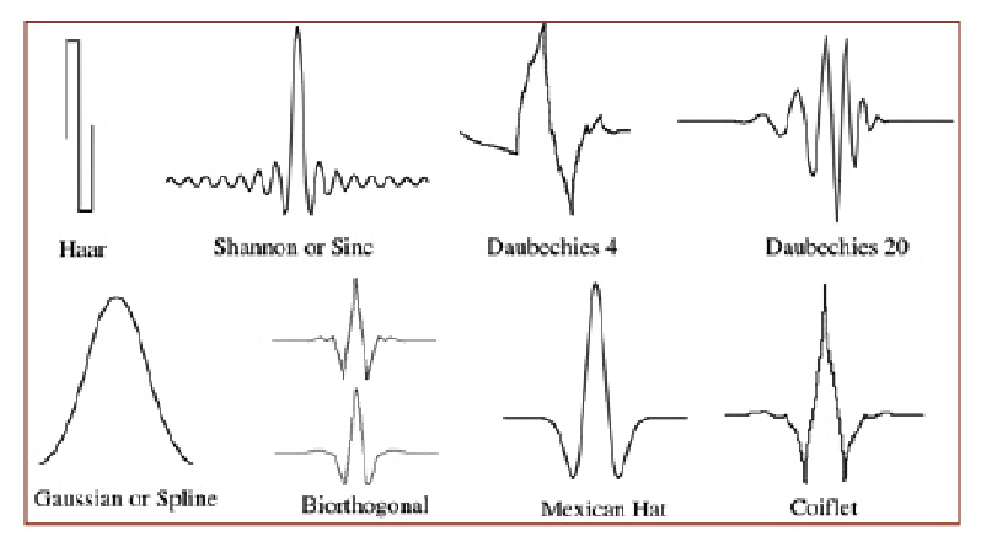
\includegraphics[scale=1.00]{graficos/ondaletas}
	\captionof{figure}{Exemplos de tipos de wavelets}
 	
\end{center}

Em seu trabalho \citeonline{Komodakis} diz que problemas de analise de imagens podem ser formulados como problemas de rotulagem, onde a partir de uma imagem segmentada, são realizadas comparações entre pontos vizinhos a fim de rotular um grupo de pontos afins. Uma questão que vem incentivando pesquisas nessas áreas, é como resolver problemas desse tipo de forma eficiente e precisa. O autor propõe a utilização do esquema primal- dual da programação linear, e diz que essa utilização revelou excelentes resultados

\subsection{Aplicações em Programação Distribuída}
Em \citeonline{Slyke} e \citeonline{Yarmish-Distrubuido} demonstram a eficiência da utilização do método simplex padrão de forma distribuída. Esse tipo de implementação é útil para a computação distribuída. Já que nesse tipo de implementação as colunas das matrizes, onde são armazenados os dados, são distribuídas entre os processadores, é mais intuitivo o uso do método simplex padrão. Além disso, esse método é mais utilizado e mais eficiente que o método revisado na resolução de problemas de grande porte, onde existe um maior volume de dados, fazendo mais sentido a utilização da programação distribuída.
De acordo com \citeonline{Slyke} e \citeonline{Yarmish-Distrubuido} a eficiência do método simplex revisado é afetada pela densidade do problema, ou seja, é uma método mais eficiente para problemas esparsos, os quais são mais comuns. Porém existem aplicações que exigem modelos mais densos, como em processamento de imagens. Nesse caso a implementação de uma algoritmo do método simplex padrão distribuído se mostra mais eficiente. Além disso, não existem algoritmos eficientes do método simplex revisado distribuído. Em conclusão o autor diz que a implementação apresentou bons resultados, especialmente para problemas grandes e densos.

Em \citeonline{Burger} é proposto um algoritmo simplex distribuído para problemas de programação linear degenerados e atribuições multi- agentes. Um problema de programação linear é dito degenerado se na solução uma das variáveis valer zero. O objetivo do trabalho é propor um algoritmo simplex para ser implementado em uma distribuição multi- agente, onde os a gentes devem concordar com uma solução ótima ou declarar o problema como inviável, caso não haja solução ótima.

Em seu trabalho \citeonline{Karypis} faz uma análise da performance de um algoritmo simplex paralelo em vários tipos de arquiteturas de rede, como por exemplo, redes hipercubo e redes de estações de trabalho. Nesse tipo de implementação do método simplex, os dados da matriz são distribuídos entre os processadores que compõem a rede. Como resultado preliminar o autor obteve que na rede hipercubo a velocidade da resolução dos problemas cresceu a medida que mais processadores foram incorporados, inclusive para problemas de grande porte. Já na rede de estações de trabalho, para problemas pequenos a velocidade não teve um aumento proporcional ao aumento do número de processadores, enquanto que para problemas de maior porte a velocidade aumentou de forma proporcional ao número de processadores.

De acordo com \citeonline{Akira-database} dentre as inúmeras ferramentas de programação linear existentes, existe a carência de uma ferramenta que resolva problemas de programação linear de forma integrada a um banco de dados, utilizando procedimentos armazenados em sql pre compiladas em armazenadas no banco de dados juntamente com os dados. Essa características em uma ferramenta se torna importante, principalmente, em problemas de grande porte, suprimindo o tráfego de dados já que toda alógica é executada internamente no banco de dados, e apenas o resultado final é enviado para o usuario. Na implementação apresentada por \citeonline{Akira-database} os dados do modelo a ser resolvido são armazenados como modelos relacionais, ou seja, em matrizes bi-dimensionais. Apesar das vantagens desse tipo de implementação, o autor chegou a conclusão que o tempo de execução ainda deve ser melhorado.

A programação linear também se aplica na área da saúde, em \citeonline{Alterovitz-saude} é feita uma proposta de utilização da programação linear no tratamento do câncer. 
Em um determinado tipo de tratamento são inseridos cateteres na área afetada para introduzir o medicamento necessário, porém o medicamento acaba afetado células saudáveis além das cancerígenas. Como os problemas de programação linear podem ser resolvidos como problemas determinísticos e com solução exata, \citeonline{Alterovitz-saude} propõe que a formulação de um problema de otimização para determinar o tempo de permanência dos cateteres, minimizando os desvios na quantidade da dose necessitada pelo paciente. Nos testes realizados, os resultados obtidos não foram mostraram uma vantagem significativa em relação ao método atualmente utilizado.

Outros exemplos bastante realistas da utilização da programação linear são os problemas de planejamento de produção e controle de estoque e os mitura. Os problemas do primeiro tipo possuem inúmeras aplicações, desde a alocação de máquinas para atender determinada demanda, até a utilização do estoque para atender a uma mudança imprevisível na demanda e necessidades de contratação de demissão para enfrentar mudanças nas necessidades de mão de obra. Já os problemas de msitura tratam, basicamente, da mistura de diferentes matérias para a produção de produtos, que devem obedecer a algumas especificações e, ao mesmo tempo, minimizar o custo ou maximizar o lucro.  \cite{Taha}.
Um exemple mais prático seria a produção de rações animais onde o objetivo é minimizar o custo de produção da ração compsta pos dois ingredientes. Estando restrito a quantidade total que deve ser produzida, além das quantidades de nutrientes necessários.

 $\\Minimize\ z=0,9x_{1}+0,5x_{2}\\
Sujeito\ a\\$
\begin{eqnarray*}
        x_{1}+x_{2}\geq 90 \ (a)\\
        0,09x_{1}+0,05x_{2}\geq 0,07(x_{1}+x_{2}) \ (b)\\
        0,02x_{1}+0,06x_{2}\geq 0,03(x_{1}+x_{2}) \ (c)\\
         x_{1}\geq 0 \ (d)\\
	 x_{2}\geq 0 \ (e)
\end{eqnarray*}

Onde, 
\begin{itemize}
\item \textbf {x1} representa a quantidade do ingrediente 1 que a ração deve conter
\item \textbf {x2} representa a quantidade do ingrediente 2 que a ração deve conter
\item \textbf {Z} representa o custo total da produção dessa ração, sendo que o custo (por grama) do ingrediente 1 é de R\$ 0,9 e o custo (por grama) do ingrediente 2 é de R\$ 0,5
\end{itemize}

E as restrições representam as restrições das quantidades de nutrientes que a ração deve conter e a quantidade total,
\begin{itemize}
\item \textbf {(a)} representa a quantidade total de ração que deve ser produzida (em quilos)
\item \textbf {(b)} representa que a ração deve conter 7\% de um determinado nutriente, e 9\% de cada grama do ingrediente 1 e 5\% de cada grama do ingrediente 2 é composto por esse nutriente. 
\item \textbf {(c)} representa que a ração deve conter 3\% de um determinado nutriente, e 2\% de cada grama do ingrediente 1 e 6\% de cada grama do ingrediente 2 é composto por esse nutriente.
\item \textbf {(d)} representa que a ração deve conter o ingrediente 1
\item \textbf {(e)} representa que a ração deve conter o ingrediente 1
\end{itemize}

A programação linear além de estar presente, é fundamental em diversas áreas, tornando-se uma ferramenta de apoio a decisão e contribuindo para o sucesso de projetos nas áreas em que se aplica.

\section{Ferramentas de Programação Linear}
Durante a pesquisa foram utilizadas e encontradas algumas ferramentas para a resolução de problemas de programação linear, além de bibliotecas com problemas testes. 
Uma das ferramentas é o Tora \cite{Taha}, que é software com uma interface simples, mas com algumas características que não há tornam muito amigável, além disso é um software mais educacional, inclusive com o recurso que mostra o passo a passo na resolução do problema utilizando o método simplex tabular.

\begin{center}
	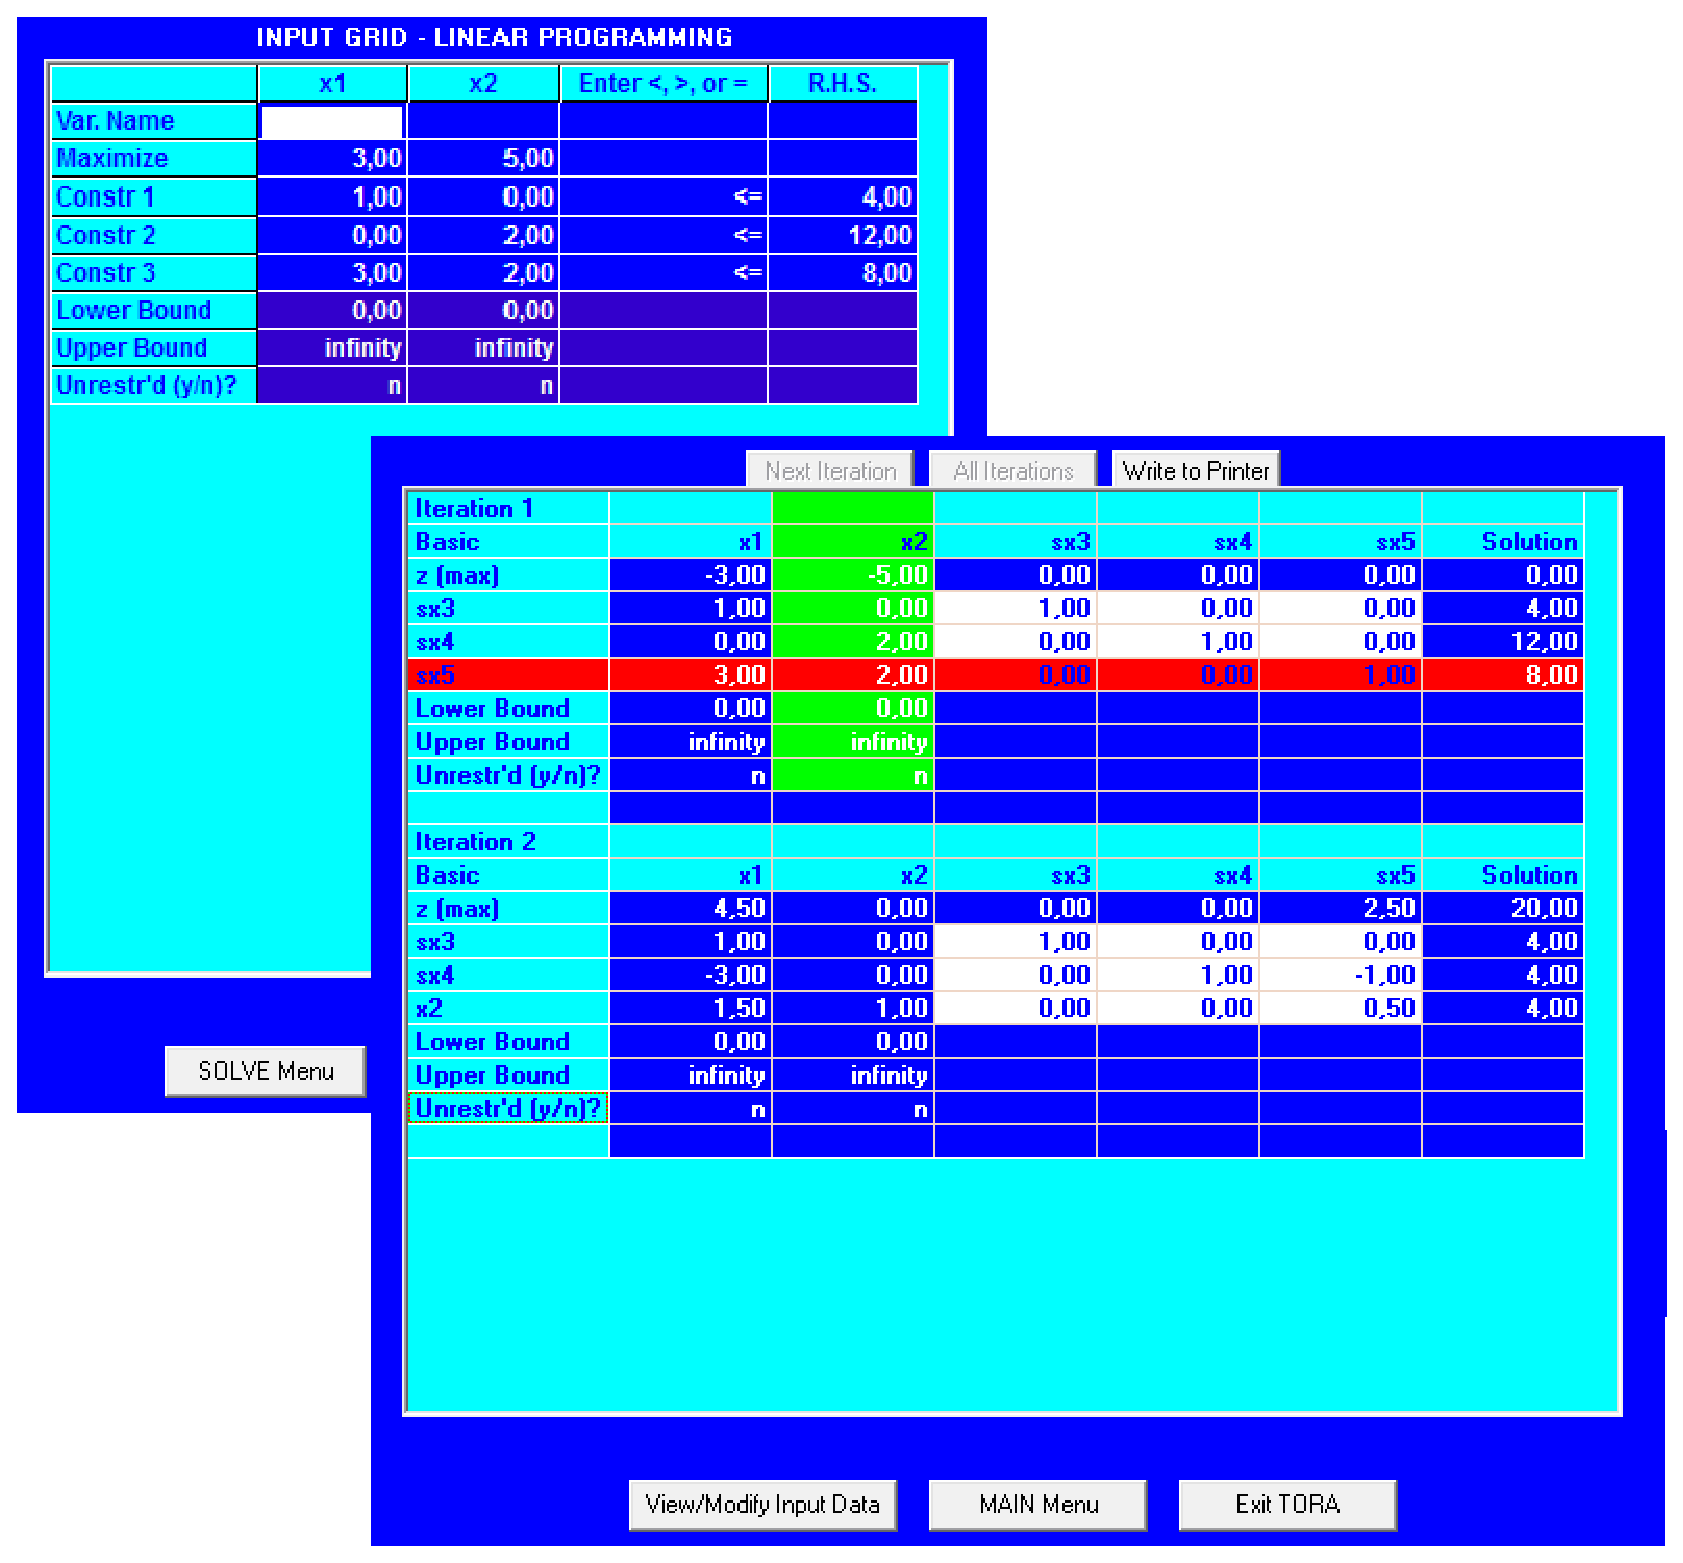
\includegraphics[scale=1.00]{tora}
	\captionof{figure}{Telas de entrada e sáida de dados do software Tora}
\end{center}

Já o Lingo disponibiliza uma versão demo gratuita. A maior dificuldade na utilização dessa ferramenta é o fato do usuário precisar digitar o modelo sem nenhuma orientação em relação a sintaxe, além disso a forma como o resultado é exibido dificulta a interpretação.
O Cplex é uma ferramenta mais robusta, com mais recursos e uma interface mais elaborada. Não é gratuita, mas uma versão com licença acadêmica é disponibilizada. Permite a modelagem e resolução de problemas de otimização de diversa natureza, como por exemplo: programação inteira, programação linear e programação inteira mista. Utilizando para isso diferentes métodos de solução.
O Glpk é um conjunto de rotinas destinadas a resolução de problemas de programação linear, além de problemas de programação inteira mista. As rotinas são escritas em ANSI C e podem ser utilizadas como biblioteca.
